\section{Réseau de neurone}

\subsection{Visualisation des données}

Pour ce TP, on se basera sur le même ensemble de données que pour le TP2. Pour débuter, on appliquera la méthode de propagation avant, couramment appelé \textit{feedforward propagation} sur la matrice $X$. Nous avons 5000 échantillons d'entrainement, où chaque échantillon représente une image d'un chiffre en niveau de gris de $20x20$px. Ce qui nous donne finalement une matrice de dimension 
5000 sur 400. \\
Dans un premier temps, nous allons en afficher une centaine de manière aléatoire à l'aide du script donné. Chaque visualisation est différente.

\begin{figure}[!h]
    \begin{center}
        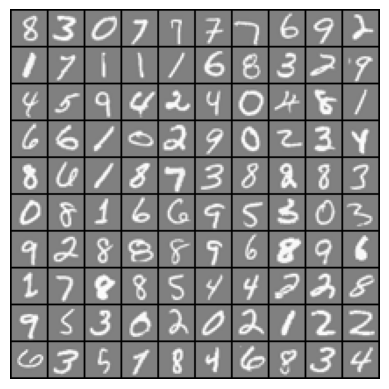
\includegraphics[width=0.4\textwidth]{./img/1.2.png}
        \caption{\label{fig:1.2}Visualisation des données}  
    \end{center}
\end{figure}



\clearpage

\subsection{Représentation du modèle}

Dans cette partie, nous allons implémenter l'architecture de réseau de neurone de la figure \ref{fig:1.1}. 
Les données d'entrainement sont chargées dans les variables X et y, tandis que les paramètres de réseau $\theta_1$ 
et $\theta_2$ ont déjà été entraînés et sont optimales pour effectuer l'exercice.

\begin{figure}[!h]
    \begin{center}
        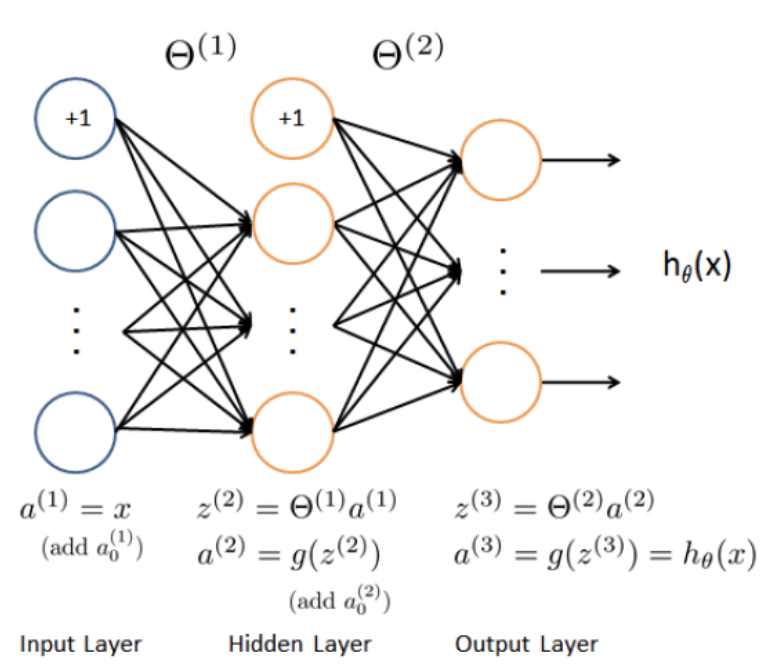
\includegraphics[width=.75\textwidth]{./img/1.1.png}
        \caption{\label{fig:1.1}Neural network model}
    \end{center}
 \end{figure}

 

L'objectif est donc d'appliquer la méthode de \textit{feedforward propagation}, 
cette méthode permettra de renvoyer la prédiction d'un réseau neuronal. Une fois implémenter, lors de 
l'appelle de la fonction \ref{lst:predictNeuralNetwork} comme dans la stratégie de classification \textit{One-Vs-All}, 
la prédiction du réseau neuronal sera l'étiquette qui a la plus grande sortie $h_{\theta}((x))_k$. \\

\noindent
La différence avec une régression logistique multi-classe est que le réseau de neurones sera capable de représenter des modèles 
complexes qui forment des hypothèses non linéaires, ce qui n'est donc pas le cas pour la régression. 

\clearpage

\subsection{Implémentation}

\begin{figure}[!h]
    \begin{minted}[frame=lines, framesep=2mm, baselinestretch=1.2, fontsize=\footnotesize, linenos, breaklines=true]{python}
    def predictNeuralNetwork(Theta1, Theta2, X):

    # Useful values
    m, _ = X.shape
    num_labels, _ = Theta2.shape
    # Input Layer
    a1 = X

    # Hidden Layer
    z2 = a1 @ Theta1.T
    a2 = sigmoid(z2)
    
    # Add column 1's to the matrix X 
    a2 = np.hstack((np.ones((X.shape[0], 1)), a2))

    # Output Layer
    z3 = a2 @ Theta2.T
    hypothesis = np.argmax(sigmoid(z3), axis=1) + 1 
    
    return hypothesis

    """return 
    Training Set Accuracy: %f 97.52
    Expected training Set Accuracy: 97.5%
    """
    \end{minted}   
    \captionof{listing}{\label{lst:predictNeuralNetwork}predictNeuralNetwork}
    \end{figure}

Ainsi, on obtient la précision et l'affichage de chaque digit de l'ensemble d'entrainement avec 
leur étiquette associée. Voici quelques exemples visibles ci-dessous. 


 \begin{figure}[!h]
     \begin{minipage}{.48\linewidth}
         \begin{center}
             
\includegraphics[width=0.55\textwidth]{./img/1.30.png}
             \caption{\label{fig:1.30}Neural prediction network: digit 5}  
         \end{center}
     \end{minipage}\hfill
     \begin{minipage}{.48\linewidth}
         \begin{center}
             
\includegraphics[width=0.55\textwidth]{./img/1.31.png}
             \caption{\label{fig:1.31}Neural prediction network: digit 2}  
         \end{center}
     \end{minipage}
 \end{figure}

   
\clearpage

















    

   

   


